\documentclass[a4paper,10pt]{article}
\setlength{\parindent}{0ex}
\setlength{\parskip}{1.5ex}
\usepackage[dvips]{graphicx}
\usepackage {epsfig}
\usepackage[a4paper, hmargin=25mm, vmargin=20mm, nohead]{geometry}

\begin{document}
\newcommand{\testmarks}[1]
{\begin{flushright}{\bf (#1 marks)}\end{flushright}}

{\centering \large \bf THE UNIVERSITY OF WAIKATO\\}
{\centering \large \bf Department of Computer Science\\[0.5cm]}

{\centering \large \bf COMP201B Computer Systems 2005\\}
{\centering \large \bf Exercise 4,5 \& 6 Test - 19th September 2005\\[0.3cm]}
{\centering \bf Worth 17\% --- Marked out of: 40\\[0.3cm]}
{\centering \bf Time allowed: 60 Min\\[1cm]}
\hrule

\begin{enumerate}
\item  In Exercise 4 you used \emph{WRAMPsim} to simulate the
execution of WRAMP instructions on a WRAMP data-path. Figure
\ref{fig:wrampblok} shows the architecture of the WRAMP CPU that
you used in the Exercise. Although not shown on the diagram there are
control lines between the control unit and each of the components,
which are used to control the flow of data on the data-path. The
control signals for each of the components and their functionality is
defined in Tables \ref{table:signals} and
\ref{table:alu} of Appendix \ref{cntrl_sig_defn}. 

\begin{figure}[h]
\begin{center}
    \psfig{figure=datapath.eps, width=.8\linewidth}
    \caption{Data-path Architecture for WRAMP CPU}
    \label{fig:wrampblok}
  \end{center}
\end{figure}

The signals used for two consecutive instructions are given in the Operation History in figure~\ref{fig:hist}.

\begin{figure}[h]
\begin{small}
\begin{center}
\begin{verbatim}
pc_out, mem_read, ir_in
pc_out, alu_out, alu_func=inc, pc_in
a_out, sel_a=$0, b_out, sel_b=$0, alu_out, alu_func=add, c_in sel_c=$1

pc_out, mem_read, ir_in
pc_out, alu_out, alu_func=inc, pc_in
a_out, sel_a=$0, b_out, sel_b=$1, alu_func=add
pc_out, imm_20_out, alu_out, alu_func=add, pc_in

 
\end{verbatim}
%% $
\end{center}
\end{small}
\caption{Operation History}
\label{fig:hist}
\end{figure}

Use the Operation History to work out which two instructions were executed.  Note that the second instruction used one immediate operand which was -2.



\testmarks{10} 

\newpage 

\item Provided in figure~\ref{code:badack} is some code which performs I/O operations.  Information regarding the I/O devices used is provided in the appendices.

\label{ques:badack}

\begin{enumerate}
\item Explain concisely what the overall purpose is of each of the following sections of code.  Repeating or paraphrasing the comments that are included in the code will not gain marks.  For example lines 5 - 12 are chaining in a new exception handler before the system handler. Give the details of any I/O devices being used and what they are being used for.

\begin{enumerate}
	\item Lines 14 - 20
	\item Lines 22 - 31
	\item Lines 33 - 35
	\item Lines 37 - 46
	\item Lines 53 - 61
	\item Line  63
\end{enumerate}

\testmarks{12}


\item What is the overall function of the program in figure~\ref{code:badack}?
\testmarks{4}

\item Which part(s) of the program use polled I/O?
\testmarks{2}

\item Is the exception handler fully compliant as defined in the WRAMP manual?
\testmarks{2}

\end{enumerate}

\begin{figure}[p]
\begin{footnotesize}
\begin{center}
\begin{tabular}{|p{12cm}|}
\hline
\begin{verbatim}
   1:   .text
   2:   .global main
   3:   main:
   4:   
   5:           # Get old exception vector handler
   6:           movsg   $4,  $evec
   7:           # Save it
   8:           sw      $4,  old_vector($0)
   9:          # Get address of our handler
   10:          la      $4,  handler
   11:          # Put in exception vector
   12:          movgs   $evec,  $4
   13:  
   14:          # Make sure there are no outstanding interrupts
   15:          sw $0, 0x70004($0)
   16:          # get current status
   17:          lw      $4,  0x70002($0)
   18:          # enable interrupts
   19:          ori     $4,  $4, 0x100
   20:          sw      $4,  0x70002($0)
   21:  
   22:          # Get control register
   23:          movsg   $4,  $cctrl
   24:          # Disable all interrupts (bits 4-11)
   25:          andi    $4,  $4,  0xf
   26:          # Enable interrupt bit
   27:          ori     $4,  $4,  0x100
   28:          # Set IE on
   29:          ori     $4,  $4,  0x2
   30:          # Store to control register
   31:          movgs   $cctrl,  $4
   32:  
   33:  loop:
   34:          # Loop indefinitely
   35:          j       loop
   36:  
   37:  handler:
   38:          # Get Status Register
   39:          movsg   $13,  $estat
   40:          # mask interrupt bit
   41:          andi    $13,  $13, 0xfef0
   42:          # If no others are set, branch to my handler
   43:          beqz    $13,  my_handle
   44:          # else load old handler
   45:          lw      $13,  old_vector($0)
   46:          jr      $13
   47:  
   48:  my_handle:
   49:          # acknowledge interrupt
   50:          sw      $0, 0x70004($0)
   51:          # get data
   52:          lw      $4, 0x70001($0)
   53:  t_check:
   54:          # Get serial port status
   55:          lw      $13,  0x71003($0)
   56:          # check if TDS bit is set
   57:          andi    $13,  $13, 0x2
   58:          # If not check again
   59:          beqz    $13, t_check
   60:          # Else transmit reg 4
   61:          sw      $4,  0x71000($0)
   62:  
   63:          rfe
   64:  
   65:  old_vector:
   66:          .word 0

\end{verbatim}
\\ \hline
\end{tabular}
\end{center}
\end{footnotesize}
\caption{Code for Question~\ref{ques:badack}}
\label{code:badack}
\end{figure}

\item Code can be added to that in figure~\ref{code:badack} to allow the system to check for changes to the switches connected to the parallel input without using the main loop.     Using the
specifications of the Parallel Interface given in Appendix~\ref{appen:parallel},
the CPU Control Register given in Appendix~\ref{appen:cctrl} and the Exception
Status Register give in Appendix~\ref{appen:estat}:

\begin{enumerate}

\item Write the changes required to the setup code to also enable interrupts from the Parallel Interface on switch changes.  Do not remove any of the existing set up conditions.

\testmarks{5}

\item Rewrite the handler to check for interrupts from the Parallel
Interface and jump to \\
 \texttt{handle\_parallel\_interrupt} as well as make the existing checks and jumps. 

\testmarks{5}

\end{enumerate}

\end{enumerate}

\newpage
\appendix
\section{Definition of the WRAMP Control Signals for Question 1} 
\label{cntrl_sig_defn}

\begin{table}[h]
\begin{center}
\begin{tabular}{|l|l|p{8cm}|}
\hline
\textbf{Component} & \textbf{Signal Name} & \textbf{Description} \\
\hline
Register File & \texttt{a\_out} & Causes the contents of the
register selected by \texttt{sel\_a} to be output onto the A bus. \\
\cline{2-3}
& \texttt{sel\_a} & Select which register will be output onto the A bus
if \texttt{a\_out} is asserted. \\
\cline{2-3}
& \texttt{b\_out} & Causes the contents of the
register selected by \texttt{sel\_b} to be output onto the B bus. \\
\cline{2-3}
& \texttt{sel\_b} & Select which register will be output onto the B bus
if \texttt{b\_out} is asserted. \\
\cline{2-3}
& \texttt{c\_in} & Causes the value from the C bus to be written
into the register selected by \texttt{sel\_c}.\\
\cline{2-3}
& \texttt{sel\_c} & Select which register to write the value from the C
bus into when the \texttt{c\_in} signal is asserted. \\
\hline
ALU & \texttt{alu\_out} & Causes the result of the current ALU function 
selected by \texttt{alu\_func} to be output to the C bus. \\
\cline{2-3}
& \texttt{alu\_func} & Defines the current operation that the ALU
should perform. ALU functions are defined in table~\ref{table:alu}. \\
\hline
Memory Interface & \texttt{mem\_read} & Causes the contents of the
memory address specified on the A bus to be read and output onto the C
bus. \\
\cline{2-3}
& \texttt{mem\_write} & Causes the value on the B bus to be written
into the memory address specified on the A bus. \\
\hline
Program Counter & \texttt{pc\_out} & Causes the contents of the PC
register to be output onto the A bus. \\
\cline{2-3}
& \texttt{pc\_in} & Causes the value on the C bus to be written into
the PC. \\
\hline
Instruction Register & \texttt{imm\_16\_out} & Causes the least
significant 16 bits of the IR to be output onto the B bus. \\
\cline{2-3}
& \texttt{imm\_20\_out} & Causes the least
significant 20 bits of the IR to be output onto the B bus. \\
\cline{2-3}
& \texttt{sign\_extend} & Causes the output from the IR to be sign
extended to 32bits. \\
\cline{2-3}
& \texttt{ir\_in} & Causes the value on the C bus to be written into
the IR. \\
\hline
Temporary Register & \texttt{temp\_out} & Causes the contents of the
temporary register to be output onto the A bus. \\
\cline{2-3}
& \texttt{temp\_in} & Causes the value on the C bus to be written into
the temporary register. \\
\hline
\end{tabular}
\end{center}
\caption{Descriptions of each of the control signals}
\label{table:signals}
\end{table}
\newpage
\begin{table}[h]
All arithmetic and test/set operations have both signed and unsigned
variants. The unsigned variant is indicated by an operation with a
'u' suffix. A signed variant treats all inputs as signed integers while
the unsigned variant treats inputs as unsigned integers.

\begin{center}
\begin{tabular}{|l|l|l|p{75mm}|}
\hline
\textbf{Type} & \textbf{Name} & \textbf{Function} 
& \textbf{Description} \\
\hline
Arithmetic & \texttt{add, addu} & A + B & Perform an integer
addition between A and B. \\
\cline{2-4}
& \texttt{sub, subu} & A - B & Perform an integer
subtraction between A and B. \\
\cline{2-4}
& \texttt{mult, multu} & A * B & Perform an
integer multiplication between A and B. \\
\cline{2-4}
& \texttt{div, divu} & A / B & Perform an integer
division between A and B. \\
\cline{2-4} 
& \texttt{rem, remu} & A $\bmod$ B & Obtain the remainder from an
integer division between A and B. \\
\hline
Bitwise & \texttt{sll} & A $<<$ B & Shift the value on A left by the number of
places specified by B. Fill with zeros. \\
\cline{2-4}
& \texttt{and} & A AND B & Perform a bitwise AND between A and B. \\
\cline{2-4}
& \texttt{srl} & A $>>$ B & Shift the value on A right by the number of places
specified by B. Fill with zeros. \\
\cline{2-4}
& \texttt{or} & A OR B & Perform a bitwise OR between A and B.\\
\cline{2-4}
& \texttt{sra} & A $>>$ B & Shift the value on A right by the number of places
specified by B. Fill with MSB.\\
\cline{2-4}
& \texttt{xor} & A XOR B & Perform a bitwise XOR between A and B. \\
\hline
Test/set & \texttt{slt, sltu} & out = 1 if ( A $<$ B) & Set out if A
is less than B\\
& & else out = 0 & \\
\cline{2-4}
& \texttt{sgt, sgtu} & out = 1 if ( A $>$ B) & Set out if A
is greater than B \\
& & else out = 0 & \\
\cline{2-4}
& \texttt{sle, sleu} & out = 1 if ( A $\le$ B) & Set out if A
is less than or equal to B\\
& & else out = 0 & \\
\cline{2-4}
& \texttt{sge, sgeu} & out = 1 if ( A $\ge$ B) & Set out if A
is greater than or equal to B\\
& & else out = 0 & \\
\cline{2-4}
& \texttt{seq, sequ} & out = 1 if ( A $=$ B) & Set out if A
is equal to B \\
& & else out = 0 & \\
\cline{2-4}
& \texttt{sne, sneu} & out = 1 if ( A $\neq$ B) & Set out if A
is not equal to B \\
& & else out = 0 & \\
\hline
Misc & \texttt{lhi} & out\tiny$_{[31...16]}$\normalsize~= B\tiny$_{[15...0]}$ &
Set the upper 16 bits of out to be the lower 16 \\
& & out\tiny$_{[15...0]}$\normalsize~= 0 & bits of B. Lower 16 bits of out set to zero. \\ 
\cline{2-4}
& \texttt{inc} & out = A + 1 & Increment A\\
\hline
\end{tabular}
\end{center}
\caption{ALU Operations}
\label{table:alu}
\end{table}

\newpage
\section{\$cctrl - CPU Control Register}
\label{appen:cctrl}
\begin{figure}[h]
\begin{center}
\includegraphics[width=\textwidth]{cctrl.eps}
\caption{\$cctrl - CPU Control Register}
\label{cctrl_pic}
\end{center}
\end{figure}

The CPU control register controls almost all of the functionality
related to the WRAMP exception mechanism. There are three main
sections of this register:

\begin{itemize}
\item Interrupt Enable (IE)
\item Kernel/User Mode (KU)
\item Interrupt Mask
\end{itemize}

\subsection{Interrupt Enable}

This flag provides a global interrupt enable. If this location is set
to `\texttt{0}' then no interrupts can be triggered. This flag
\emph{only} affects external interrupts. There is no way on the WRAMP
processor to disable internal exceptions.

Interrupts that occur while the global interrupt enable is turned off
will be held back. As soon as interrupts are again enabled by writing
a `\texttt{1}' into this location the interrupt mask will be consulted
to discover if that specific interrupt is enabled. See
Section~\ref{sec:imask} for more information about the interrupt mask.

The CPU will automatically set the IE bit to `\texttt{0}' whenever an
exception of any type occurs. This prevents the exception handler
from being interrupted by another interrupt.

\subsection{Interrupt Mask}
\label{sec:imask}

This provides a way to selectively turn on and off individual external
interrupts. This field has a bit corresponding to each of the eight
possible external interrupts (IRQ0 - IRQ7). Bit 4 of the CPU control
register corresponds to IRQ0, bit 5 to IRQ1 and so on.

The interrupt mask field is only consulted if the global interrupt
enable (IE) flag is set. If an interrupt occurs and the global
interrupt flag is set but the individual interrupt mask is disabled
then the interrupt will be held back. As soon as both the global
interrupt enable and the specific interrupt mask bits are set then the
interrupt will occur.

\subsection{Kernel User Mode}

The WRAMP CPU has two modes of operation, kernel and user mode. If
there is a `\texttt{1}' in the KU bit the CPU is in kernel mode. If
the KU bit is set to `\texttt{0}' then the CPU is in user mode. 

If the CPU is running in kernel mode it will execute all instructions and
allow access to all areas of memory. If the CPU is running in user
mode programs are not allowed to use any of the three instructions
which deal with the special register file (\texttt{movsg, movgs, rfe})
and may not be able to access all memory locations. If a program
running in user mode attempts to use one of these instructions, or to
access protected memory the CPU will cause a General Protection Fault
exception.

The CPU will automatically set the KU bit to `\texttt{1}' whenever an
exception of any type occurs. This allows the exception handler to
operate in kernel mode, allowing it full access to all instructions
and memory locations.

\newpage
\section{\$estat - Exception Status Register}
\label{appen:estat}

\begin{figure}[h]
\begin{center}
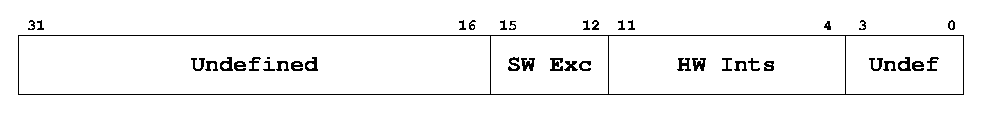
\includegraphics[width=\textwidth]{estat.eps}
\caption{\$estat - Exception Status Register}
\label{estat_pic}
\end{center}
\end{figure}

The exception status register provides the exception handler with the
ability to discover what exceptions caused it to be called. The
exception status register has a single bit flag for each external IRQ
line. Bit 4 of the status register corresponds to IRQ0, bit 5 to IRQ 1
and so on. In addition to the eight external interrupt sources the
status register also provides the status for the four CPU internal
exception sources.

The full list of all exception sources and their related status
register bit is given in Table~\ref{table:sta_loc}.

\begin{table}[h]
\begin{center}
\begin{tabular}{|l|c|}
\hline
\textbf{Exception source} & \textbf{Bit location} \\
\hline
IRQ0 & 4 \\
\hline
IRQ1 - User Interrupt Button & 5 \\
\hline
IRQ2 - Timer Interrupt & 6 \\
\hline
IRQ3 - Parallel Interrupt & 7 \\
\hline
IRQ4 - Serial Port 1 Interrupt & 8 \\
\hline
IRQ5 - Serial Port 2 Interrupt & 9 \\
\hline
IRQ6 & 10 \\
\hline
IRQ7 & 11 \\
\hline
General Protection Fault Exception & 12 \\
\hline
System Call Exception & 13 \\
\hline
Breakpoint Exception & 14 \\
\hline
Arithmetic Exception & 15 \\
\hline
\end{tabular}
\caption{Exception Status Register Fields}
\label{table:sta_loc}
\end{center}
\end{table}


\newpage
\section{Details of the Serial ports}
\label{org_sp_defn}



The REX board provides two serial interfaces, one of which is
connected to the Linux machine and the other is connected to the
terminal that should be sitting on the shelf above the board. 

For each of the serial interfaces there are 4 registers accessible to
the CPU. These registers are the transmit data register, the receive
data register, the status register and the control register.

The transmit data register holds the value that is to be sent out of
the serial port. The receive data register holds the value that has
been received in the serial port. The status register indicates if
there is a value in the receive data register and also if the value in
the transmit data register has been sent. The control register allows
the configuration of the serial port. For this Exercise the control
register will have already been configured for you by the monitor so
it will not need to be altered. Each serial port has a base address
and the 4 registers for each serial port are expressed as an offset
from this address. The base addresses for each port are defined in
table~\ref{table:serialbase} and the offsets are defined in
table~\ref{table:serialoffset}. The format of the status register for
each of the serial devices is shown in table~\ref{table:serialstat}.

\begin{table}[h]
\begin{center}
\begin{tabular}{|l|l|}
\hline
\textbf{Port} & \textbf{Base Address} \\
\hline
Linux machine & 0x70000 \\ 
\hline
Terminal & 0x71000 \\
\hline
\end{tabular}
\end{center}
\caption{Base addresses for each serial port}
\label{table:serialbase}
\end{table}

\begin{table}[h]
\begin{center}
\begin{tabular}{|l|c|}
\hline
\textbf{Register name} & \textbf{Offset} \\
\hline
Serial Transmit Data Register & 0 \\
\hline
Serial Receive Data Register & 1 \\
\hline
Serial Control Register & 2 \\
\hline
Serial Status Register & 3 \\
\hline
Serial Interrupt Acknowledge Register & 4 \\
\hline
\end{tabular}
\caption{Serial Port Register Offsets}
\label{table:serialoffset}
\end{center}
\end{table}

\begin{table}[h]
\begin{center}
\begin{tabular}{|l|l|}
\hline
\textbf{Bit} & \textbf{Function} \\
\hline
0 & Receive Data Ready \\
 & 1 if data in receive data register, 0 otherwise \\
\hline
1 & Transmit Data Sent \\
 & 1 if ready for next character, 0 if data is still being transmitted  \\
\hline
\end{tabular}
\end{center}
\caption{Status register format}
\label{table:serialstat}
\end{table}

\subsection{Serial Control Register}

This register allows line parameters such as serial bit rate to be
set. The serial ports are configured appropriately by the monitor for
the device setup used by the Computer Systems course. Unless you know
that you specifically need to change something in this register you
should leave it as default.

The control register also controls when the serial port will cause an
interrupt. The serial port can selectively cause an interrupt when a
character is received into the receive data register, the transmit
data register becomes empty or on an error condition. Any combination of
these can be enabled or disabled at one time. To enable interrupts to
be used by the serial port under specific circumstances a `\texttt{1}'
should be written to the appropriate location. If an interrupt has
occurred it must be acknowledged by writing into the serial interrupt
acknowledge register.

The REX board monitor will initialise the serial port so that no
interrupts are enabled

The control register is a read/write register. Writes to this register
have an immediate effect on the line settings.

\begin{figure}[h]
\begin{center}
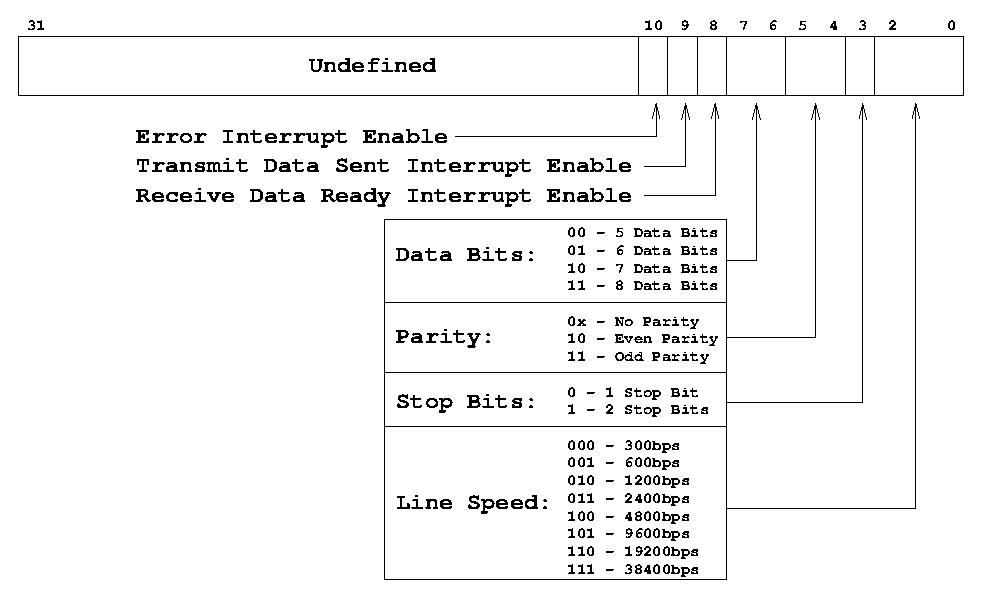
\includegraphics[width=0.8\textwidth]{serial_cr.eps}
\caption{The Serial Control Register}
\label{serial_cr_pic}
\end{center}
\end{figure}

\noindent
eg. To configure a serial interface to operate with no interrupts
enabled, at 9600 bits per second, with 8 data bits, no parity and 1
stop bit, the value `\texttt{00011000101}' would be written to the
control register.

\subsection{Serial Interrupt Acknowledge Register}

The interrupt acknowledge register is a read/write register. When the
serial interface has generated an interrupt this register allows the
program to determine the reason for the interrupt as well as
acknowledge interrupts that have been dealt with.

To acknowledge an interrupt a zero (`\texttt{0}') should be written
over the current status field for the type of interrupt being
acknowledged. Most often it will be the desire of the programmer to
acknowledge all of the possible serial port interrupts in one
instruction. This can be achieved by storing register \texttt{\$0} to
the interrupt acknowledge register.

\begin{figure}[h]
\begin{center}
\includegraphics[width=0.8\textwidth]{serial_iack.eps}
\caption{The Serial Interrupt Acknowledge Register}
\label{serial_iack_pic}
\end{center}
\end{figure}

\clearpage
\newpage
\section{Parallel Interface}
\label{appen:parallel}
The parallel interface on the REX board provides an input interface
from a bank of 8 on-off switches and two momentary push-buttons, as
well as an output interface to two LED Seven Segment Displays (SSDs).
Parallel interrupts, if enabled, will be generated on any switch or
push-button state change.

The programmers view of the parallel interface consists of six
registers.  The names of these registers and their addresses,
expressed as offsets from the base address, are provided in
Table~\ref{table:parallel_offsets}. The base address for the parallel
port is \texttt{0x73000}.

\begin{table}[h]
\begin{center}
\begin{tabular}{|l|c|}
\hline
\textbf{Register name} & \textbf{Offset} \\
\hline
Parallel Switch Register & 0 \\
\hline
Parallel Push Button Register & 1 \\
\hline
Parallel Left SSD Register & 2 \\
\hline
Parallel Right SSD Register & 3 \\
\hline
Parallel Control Register & 4 \\
\hline
Parallel Interrupt Acknowledge Register & 5 \\
\hline
\end{tabular}
\caption{Parallel Port Register Offsets}
\label{table:parallel_offsets}
\end{center}
\end{table}



\subsection{Parallel Switch Register}

The switch register is a read-only register. A read from this register
returns a bit pattern with bits set corresponding to the switches that
are on.

\begin{figure}[h]
\begin{center}
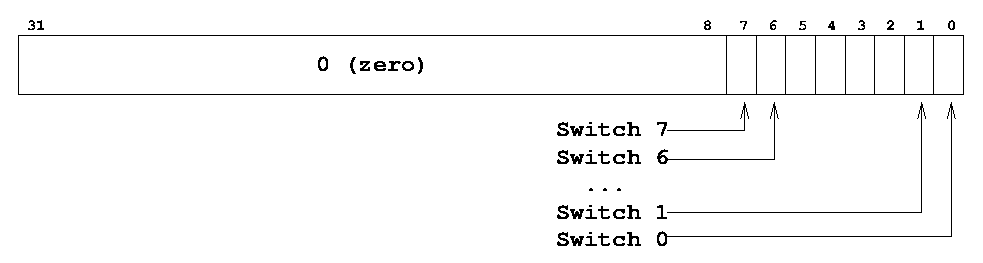
\includegraphics[width=0.8\textwidth]{switch_reg.eps}
\caption{The Switch Register}
\label{switch_reg_pic}
\end{center}
\end{figure}


\subsection{Parallel Push Button Register}

The push button register is a read-only register. A read from this
register returns a bit pattern in the low order 2 bits corresponding
to the push buttons that are currently being depressed.

\begin{figure}[h]
\begin{center}
\includegraphics[width=0.8\textwidth]{button_reg.eps}
\caption{The Push Button Register}
\label{button_reg_pic}
\end{center}
\end{figure}

\subsection{Parallel Left and Right SSD Registers}

The Left and Right SSD Registers are read/write registers. These
registers contain the value to be displayed on their respective Seven
Segment Display. 

If the hexadecimal to seven-segment decode bit is enabled in the
parallel control register, four bits of input will be decoded into a
single hexadecimal digit and displayed on the seven-segment display.

If the hexadecimal to seven-segment decode bit is turned off, then
each segment can be individually controlled by a single bit of the
input. The displays are made up of seven segments and a decimal point.
The first eight bits of input turn on the segments as shown in
Figure~\ref{fig:ssd}.

\begin{figure}[h]
\begin{center}
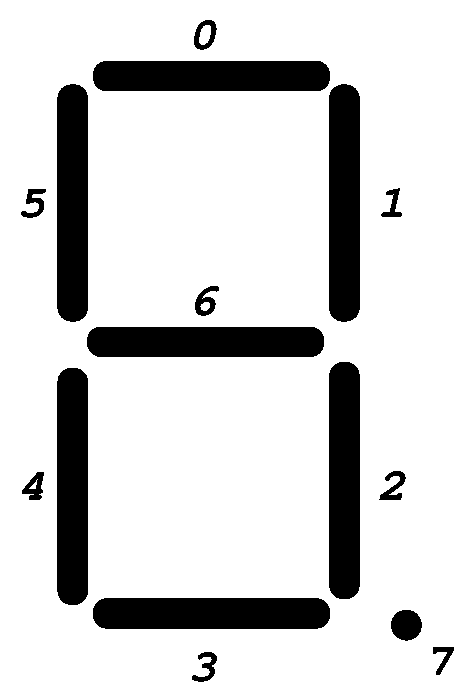
\includegraphics[width=0.12\textwidth]{ssd.eps}
\caption{Seven-segment display bit encoding}
\label{fig:ssd}
\end{center}
\end{figure}

\subsection{Parallel Control Register}

The Parallel Control Register is a read/write register, which allows
for control over the parallel interface.

\begin{figure}[h]
\begin{center}
\includegraphics[width=0.8\textwidth]{parallel_cr.eps}
\caption{The Parallel Control Register}
\label{parallel_cr_pic}
\end{center}
\end{figure}

eg. To enable interrupts on switch changes and force hex-SSD decoding
on the displays, a value of `\texttt{11}' would be written to
the parallel control register.

\subsection{Parallel Interrupt Acknowledge Register}

The Interrupt Acknowledge Register is a read/write register. This
register allows a program to determine the parallel port interrupt
status as well as acknowledge interrupts that have been dealt with.

\begin{figure}[h]
\begin{center}
\includegraphics[width=0.8\textwidth]{parallel_iack.eps}
\caption{The Parallel Interrupt Acknowledge Register}
\label{parallel_iack_pic}
\end{center}
\end{figure}

eg. To acknowledge an outstanding parallel port interrupt `\texttt{0}'
would be written to the parallel interrupt acknowledge register.

\end{document}




